%%%%%%%%%%%%%%%%%%%%%%%%%%%%%%%%%%%%%%%%%%%%%%%%%%%%%%%%%%%%%%%%%%%%%%%%%%%%%
%%%
%%% Lucrare de licență – UTCN, Facultatea de Automatică și Calculatoare,
%%% Departamentul Calculatoare.
%%% Pornește de la șablonul oficial templateLaTeX-Rom-2026 (thesis.tex v1.8).
%%%
%%% Diferențe față de șablon:
%%%  - fără xy (pachetul lipsește și nu este folosit);
%%%  - fără ae/aecompl: acestea înlocuiau fontul Times cu Computer Modern,
%%%    iar metodologia cere Times New Roman 12 pt; cu lualatex: Times New Roman
%%%    dacă există, altfel TeX Gyre Termes (aceeași formă); cu pdflatex: mathptmx;
%%%  - fără lipsum (text de umplutură); în plus tikz pentru figuri;
%%%  - fără pagina cu instrucțiuni (ghid.tex), care se elimină din versiunea finală.
%%%
%%% Compilare: latexmk licenta.tex (folosește lualatex, vezi latexmkrc)
%%%%%%%%%%%%%%%%%%%%%%%%%%%%%%%%%%%%%%%%%%%%%%%%%%%%%%%%%%%%%%%%%%%%%%%%%%%%%

\documentclass[12pt,a4paper,twoside]{report}

\usepackage{cs}
\usepackage{iftex}
\usepackage{amsmath,amsbsy}
\usepackage{amstext}
\ifPDFTeX
  % pdflatex: ș și ț sunt compuse din două glife (textul copiat din PDF devine ",s")
  \usepackage[T1]{fontenc}
  \usepackage[utf8]{inputenc}
  \usepackage{mathptmx}
  \usepackage{latexsym}
  \usepackage{amssymb}
\else
  % lualatex (implicit, vezi latexmkrc): ș și ț sunt glife reale, textul se copiază corect
  \usepackage{fontspec}
  \IfFontExistsTF{Times New Roman}
    {\setmainfont{Times New Roman}}
    {\setmainfont{TeX Gyre Termes}}
  \usepackage{unicode-math}
  \setmathfont{TeX Gyre Termes Math}
\fi
\usepackage[romanian]{babel}
\usepackage{graphicx}
\usepackage{graphics}
\usepackage{algorithm}
\usepackage{color}
\usepackage{titlesec}
\usepackage{fancyhdr}
\usepackage{tikz}
\usetikzlibrary{arrows.meta,calc,decorations.pathreplacing,patterns}
\usepackage{hyperref}
%% decomentati linia urmatoare pentru e nu mai evidenția hiper legăturile pentru imprimare pe hârtie
%\hypersetup{hidelinks}
\usepackage{geometry}
\usepackage{enumitem}

%%%%%%%%%%%%%%%%%%%%%%%%%%%%%%%%%%%%%%%%%%%%%%%%%%%%%%%%%%%%%
\setlist{noitemsep,nolistsep}


\diplomathesis
\centerchapter
\singlespace
\newenvironment{definition}[1][Definiție.]{\begin{trivlist}
\item[\hskip \labelsep {\bfseries #1}]}{\end{trivlist}}

%% notă de lucru (albastru, ca în șablon); se șterge din versiunea finală
\newcommand{\notalucru}[1]{{\color{blue}\noindent #1\\}}

%%% setari pagină
 \geometry{
	a4paper,
	total={159.2mm,246.2mm},
	left=25.4mm,
	top=25.4mm,
}


\begin{document}
%\frontmatter
%%%%%%%%%%% Stil pentru paginile de capăt
\pagestyle{fancy}
\setlength{\voffset}{-10pt}
\setlength\headheight{70.0pt}
%\addtolength{\textheight}{-80.0pt}
\renewcommand{\headrulewidth}{0pt}
\chead{%
	
\includegraphics[width=\textwidth]{figs/AntetUTCNRom.pdf}
}
\cfoot{}
\lfoot{}
\rfoot{}
%%%%%%%%%%%%%%%%%%%%%%%%%%%%%% Schimbați corespunzător ultimul element
\renewcommand{\thesisauthor}{Vlad SĂRĂNDAN}    %% Prenumele și numele dvs.
\renewcommand{\thesismonth}{Iulie}     %% Luna sesiunii de licență
\renewcommand{\thesisyear}{2027}      %% Anul sesiunii de licență
\renewcommand{\thesistitle}{TITLUL LUCRĂRII DE LICENȚĂ} % Titlul luucrării de licență
\renewcommand{\thesissupervisor}{titlul științific Prenume NUME} %% Conducătorul științific
%%%%%%%%%%%%%%%%%%%%%%%%%%%%%%%%%%%%%
\newcommand{\makeThesisTitle}{\textbf{\thesistitletypesize \thesistitle}}
\newcommand{\makeThesisType}{\thesistypetypesize \thesistype}
\newcommand{\department}{\sffamily\bfseries\small FACULTATEA DE AUTOMATICĂ ȘI CALCULATOARE\\
	DEPARTAMENTUL CALCULATOARE} 
\renewcommand{\thesistype}{LUCRARE DE LICENȚĂ}
\newcommand{\uline}[1]{\rule[0pt]{#1}{0.4pt}}
% Headings pentru folie de capăt
%%%%% Pagina cu titlul tezei nu trebuie să schimbati nimic %%%%%%%%%%%%%%%%%%%%%%%%
\begin{center}
	{\department}
	
	\vspace{4cm}
	\makeThesisTitle
	~\\~\\
	
	\makeThesisType
	
	~\\\vspace{6.5cm}
	
	\begin{tabular}{p{.3\linewidth}p{.5\linewidth}}
		{\hfill Absolvent:} & {\bf \thesisauthor} \\
		&\\
		{\parbox[t]{\linewidth}{\qquad\qquad\qquad Coordonator\\\hspace*{3.2cm}științific:}}& {\bf \thesissupervisor}\\
	\end{tabular}
	
	\vspace{3cm}
	{\bf \thesisyear}
\end{center}
%%%%%%%%%%%%%%%%%%%%%%%%%%%%%%%%%%%%%%%%%%%%%%%%%%%%%
\newpage
%%%%%%% Pagina cu tema %%%%%%%%%%%%%%%%%%%%%%%%%%%%%%%
\begin{center}
	{\department}
\end{center}
\vspace{0.5cm}

%\begin{small}
\begin{tabular}{p{7cm}p{8cm}}
	%\hspace{-1cm}& VIZAT,\\
	\hspace{-1cm}DECAN, & DIRECTOR DEPARTAMENT,\\
	\hspace{-1cm}{\bf Prof. dr. ing. Vlad MUREȘAN} & {\bf Prof. dr. ing. Rodica POTOLEA}\\  
\end{tabular}

\vspace{2cm}

\begin{center}
	Absolvent: {\bf \thesisauthor}
	
	\vspace{1cm}
	
	{\bf \thesistitle}
\end{center}

\vspace{5mm}
%%%%%%%%%%%%%%%%%%%%%%% Aici modificați
\begin{enumerate}
	\item {\bf Enunțul temei:} {\it Scurtă descriere a temei lucrării de licență și datele inițiale}
	\item {\bf Conținutul lucrării:} {\it (enumerarea părților componente) Exemplu: Pagina de prezentare, aprecierile coordonatorului de lucrare, titlul capitolului 1, titlul capitolului 2, titlul capitolului n, bibliografie, anexe.}
	\item {\bf Locul documentării:} {\it Exemplu}: Universitatea Tehnică din Cluj-Napoca, Departamentul Calculatoare
	\item {\bf Consultanți:}
	\item {\bf Data emiterii temei:} {\color{blue}de completat} %%%%%%%%%%%%% Modificați corespunzător
	\item {\bf Data predării:} {\color{blue}de completat} %%%%%%%%%%%%%%% Modificați corespunzător
\end{enumerate}
\vspace{1.2cm}

\hspace{6cm} Absolvent: \uline{6cm} 

\vspace{0.5cm}
\hspace{6cm} Coordonator științific: \uline{5cm} 
\newpage
%%%%%%%%% Pagina cu declarația
\begin{center}
	{\department}
\end{center}
\vspace{0.5cm}

\begin{center}
	{\bf Declarație pe propria răspundere privind\\ 
		autenticitatea lucrării de licență}
\end{center}
\vspace{1cm}

\begin{minipage}{\linewidth}
	Subsemnatul(a) \uline{.73\linewidth},
	\uline{.82\linewidth}
	legitimat(ă) cu\\ \uline{4cm} seria \uline{3cm} nr. \uline{6.3cm}
	(conform copiei anexate prezentei declarații, copie semnată și certificată ”conform cu originalul”), autorul lucrării\
	\uline{\linewidth}
	\uline{\linewidth}
	\uline{\linewidth}
	elaborată în vederea susținerii examenului de finalizare a studiilor de licență la Facultatea de Automatică și Calculatoare, Programul de studiu \uline{10cm} din cadrul Universității Tehnice din Cluj-Napoca, sesiunea \uline{4cm} a anului universitar \uline{3cm}, declar pe proprie răspundere, că această lucrare este rezultatul propriei activități intelectuale, pe baza cercetărilor mele și pe baza informațiilor obținute din surse care au fost citate, în textul lucrării și în bibliografie.\\
	Declar, că această lucrare nu conține porțiuni plagiate, iar sursele bibliografice au fost folosite cu respectarea legislației române și a convențiilor internaționale privind drepturile de autor.\\
	Declar, de asemenea, că această lucrare nu a mai fost prezentată în fața unei alte comisii de examen de licență.\\
	În cazul constatării ulterioare a unor declarații false, voi suporta sancțiunile administrative, respectiv, \emph{anularea examenului de licență}.
	Sunt de acord ca, pe tot parcursul vieții, în cazul în care este necesar și se va dori verificarea autenticității lucrării mele să fiu identificat și verificat în baza datelor declarate de mine și conform copiei documentului de identitate menționat mai sus.
\end{minipage}
\vspace{1.5cm}

Data \hspace{8cm} Nume, Prenume

\vspace{0.5cm}

\uline{3cm} \hspace{5cm} \uline{5cm}

\vspace{1cm}
\hspace{9.4cm}Semnătura
\newpage
 % Primele 3 pagini
\pagestyle{fancy}
\setlength\headheight{16.0pt}
\renewcommand{\chaptermark}[1]{\markboth{\chaptername~\thechapter.~#1}{}}
\renewcommand{\sectionmark}[1]{\markright{\thesection\ #1}}
\renewcommand{\headrulewidth}{0.4pt}
\lhead{}
\chead{%
	\leftmark\rightmark
}
\chead{}
\cfoot{\thepage}
\lfoot{}
\rfoot{}

%%%%%%%%%%%% Cuprinsul %%%%%%%%%%%%%%%%%%%%%%%%%%%%%%%%%%%%%%%%
\pagenumbering{roman}
\setcounter{page}{1}

\newpage

\tableofcontents

\newpage

%\listoftables
%\listoffigures

%%%%%%%%%%%%%%%%%% de aici începe numerotarea paginilor
\pagenumbering{arabic}
\setcounter{page}{1}


\titleformat{\chapter}[hang]
{\normalfont\Large\bfseries}{\chaptertitlename\ \thechapter.}{1em}{}
\titleformat{\section}[hang]
{\normalfont\large\bfseries}{\thesection.}{1em}{}
\titleformat{\subsection}[hang]
{\normalfont}{\thesubsection.}{1em}{}
\titlespacing*{\section}{0pt}{12pt}{6pt}
\titlespacing*{\subsection}{0pt}{12pt}{6pt}
\titlespacing*{\chapter}{0pt}{30pt}{18pt}

\chapter{Introducere}\label{ch:intro}
\pagestyle{fancy}

\notalucru{De scris (2--3 pagini): contextul temei și conturarea domeniului exact al temei.}
 % \chapter{Introducere}

\chapter{Obiectivele proiectului}\label{ch:obiective}
\pagestyle{fancy}

\notalucru{De scris (2--3 pagini): tema propriu-zisă, formulată exact, cu obiective clare.}
 % \chapter{Obiectivele Proiectului}

\chapter{Studiu bibliografic}\label{ch:studiubib}
\pagestyle{fancy}

\notalucru{De scris (3--10 pagini): stadiul actual al cunoașterii. Sisteme care folosesc CSI din echipamente Wi-Fi comerciale, cu avantaje și dezavantaje. Conceptele fizice sunt în capitolul~\ref{ch:analysis}; aici se citează doar ce au făcut alți autori.}
 % \chapter{Studiu Bibliografic}

\chapter{Analiză și fundamentare teoretică}
\label{ch:analysis}
\pagestyle{fancy}

Acest capitol prezintă bazele fizice și teoretice ale informației despre starea canalului (\emph{Channel State Information}, CSI) într-o rețea Wi-Fi.
Sunt descrise propagarea semnalului pe mai multe căi, reprezentarea complexă a semnalului, modulația OFDM din standardul IEEE~802.11 și modul în care receptorul estimează canalul.
Urmează efectul unei persoane asupra CSI, limitările măsurării pe echipamente comerciale și modul în care placa ESP32 pune CSI la dispoziția aplicației.
Implementarea pe placa ESP32 este descrisă în capitolul~\ref{ch:proiectare}.

Pe parcursul capitolului, mențiunea \emph{(calcul propriu)} marchează un rezultat obținut de autor din relațiile citate, iar mențiunea \emph{(deducție proprie)} marchează o concluzie a autorului care nu apare ca atare în sursă.
Mențiunea \emph{(analiză proprie)} marchează un rezultat obținut de autor prin dezasamblarea bibliotecilor ESP-IDF, metodă descrisă în capitolul~\ref{ch:proiectare}.

%--------------------------------------------------------------------
\section{Propagarea semnalului pe mai multe căi}\label{sec:multicale}

Într-o încăpere, semnalul emis ajunge la receptor pe mai multe căi: pe calea directă și prin reflexii pe pereți, podea, tavan și mobilier.
Când în încăpere se află o persoană, corpul ei introduce căi suplimentare, prin împrăștierea semnalului~\cite[Sec.~3.1]{zhang2015antifall}.
Figura~\ref{fig:multicale} ilustrează această situație.

\begin{figure}[ht]
	\centering
	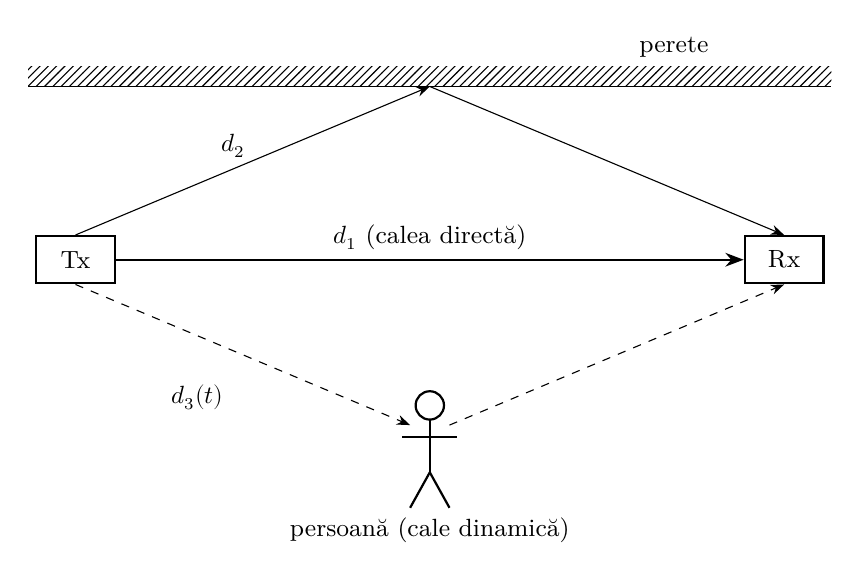
\begin{tikzpicture}[>=Stealth, font=\small]
		% perete
		\fill[pattern=north east lines] (-0.6,3.0) rectangle (9.6,3.25);
		\draw (-0.6,3.0) -- (9.6,3.0);
		\node[above] at (7.6,3.25) {perete};
		% emițător și receptor
		\node[draw, thick, minimum width=1cm, minimum height=0.6cm] (tx) at (0,0.8) {Tx};
		\node[draw, thick, minimum width=1cm, minimum height=0.6cm] (rx) at (9,0.8) {Rx};
		% calea directă
		\draw[->, thick] (tx.east) -- node[above] {$d_1$ (calea directă)} (rx.west);
		% reflexia pe perete
		\draw[->] (tx.north) -- (4.5,3.0);
		\draw[->] (4.5,3.0) -- (rx.north);
		\node at (2.0,2.25) {$d_2$};
		% persoana
		\draw[thick] (4.5,-1.05) circle (0.18);
		\draw[thick] (4.5,-1.23) -- (4.5,-1.9);
		\draw[thick] (4.15,-1.45) -- (4.85,-1.45);
		\draw[thick] (4.5,-1.9) -- (4.25,-2.35);
		\draw[thick] (4.5,-1.9) -- (4.75,-2.35);
		\draw[->, dashed] (tx.south) -- (4.25,-1.3);
		\draw[->, dashed] (4.75,-1.3) -- (rx.south);
		\node at (1.55,-0.95) {$d_3(t)$};
		\node[below] at (4.5,-2.35) {persoană (cale dinamică)};
	\end{tikzpicture}
	\caption{Propagarea pe mai multe căi într-o încăpere: calea directă ($d_1$), o reflexie pe perete ($d_2$) și o reflexie pe o persoană ($d_3(t)$). Desen propriu.}
	\label{fig:multicale}
\end{figure}

Fiecare cale $i$ are o atenuare $a_i(t)$ și o întârziere de propagare $\tau_i(t)$.
Dacă atenuările și întârzierile nu depind de frecvență în banda ocupată, semnalul recepționat $y(t)$ este suma copiilor atenuate și întârziate ale semnalului emis $x(t)$~\cite[Sec.~2.2.1]{tse2005}:
\begin{equation}\label{eq:io}
	y(t) = \sum_i a_i(t)\, x\bigl(t - \tau_i(t)\bigr).
\end{equation}
Canalul este deci un sistem liniar variabil în timp, cu răspunsul la impuls~\cite[ec.~(2.18)]{tse2005}
\begin{equation}\label{eq:h}
	h(\tau, t) = \sum_i a_i(t)\, \delta\bigl(\tau - \tau_i(t)\bigr).
\end{equation}
Întârzierea unei căi depinde de lungimea ei, $d_i(t)$, prin relația $\tau_i(t) = d_i(t)/c$, unde $c$ este viteza luminii~\cite[Sec.~3.2]{wang2015carm}.

Răspunsul în frecvență al canalului (\emph{Channel Frequency Response}, CFR) la momentul $t$ este transformata Fourier a lui $h(\tau,t)$ în raport cu $\tau$~\cite[ec.~(2.20)]{tse2005}:
\begin{equation}\label{eq:cfr}
	H(f; t) = \int_{-\infty}^{\infty} h(\tau, t)\, e^{-j2\pi f \tau}\, d\tau = \sum_i a_i(t)\, e^{-j2\pi f \tau_i(t)}.
\end{equation}
Fiecare cale contribuie cu un fazor (un număr complex) al cărui unghi depinde de frecvența $f$ și de întârzierea $\tau_i$.
Chiar dacă atenuările individuale nu depind de frecvență, răspunsul total variază cu frecvența, deoarece căile au întârzieri diferite~\cite[Sec.~2.2.1]{tse2005}.
La unele frecvențe fazorii se adună, iar la altele se anulează parțial.
Acest fenomen se numește \emph{fading selectiv în frecvență}.

Variația lui $H(f;t)$ cu frecvența depinde de dispersia întârzierilor, $T_d$ (în engleză, \emph{delay spread}).
Aceasta este diferența dintre întârzierile celei mai lungi și celei mai scurte căi cu energie semnificativă~\cite[Sec.~2.3.2]{tse2005}:
\begin{equation}\label{eq:td}
	T_d = \max_{i,j} \bigl|\tau_i(t) - \tau_j(t)\bigr|.
\end{equation}
Banda de coerență, $W_c = 1/(2T_d)$, arată pe ce interval de frecvență răspunsul canalului rămâne aproximativ constant~\cite[Tab.~2.1]{tse2005}.
Dacă banda semnalului, $W$, este mult mai mare decât $W_c$, fadingul este selectiv în frecvență~\cite[Tab.~2.2]{tse2005}.
De exemplu, o diferență de 15~m între lungimile a două căi dă $T_d = 50$~ns și $W_c = 10$~MHz, adică mai puțin decât banda de 20~MHz a unui canal Wi-Fi (calcul propriu).
Halperin et~al. arată, pe măsurători CSI reale, cât de diferit poate fi canalul de la o subpurtătoare la alta~\cite[Sec.~2]{halperin2011}.

%--------------------------------------------------------------------
\section{Reprezentarea complexă a semnalului. Componentele I și Q}\label{sec:iq}

Semnalul Wi-Fi ocupă o bandă $W$ în jurul unei frecvențe purtătoare $f_c$, de exemplu în banda de 2,4~GHz.
Majoritatea prelucrărilor din receptor (demodularea, sincronizarea, decodarea) se fac însă în banda de bază~\cite[Sec.~2.2.2]{tse2005}.
Semnalul real de radiofrecvență $s(t)$ se scrie cu ajutorul echivalentului său complex în banda de bază, $s_b(t)$~\cite[ec.~(2.23)]{tse2005}:
\begin{equation}\label{eq:banda_baza}
	s(t) = \sqrt{2}\, \mathrm{Re}\bigl\{ s_b(t)\, e^{j2\pi f_c t} \bigr\}.
\end{equation}
Partea reală a lui $s_b(t)$ se numește \emph{componenta în fază} (I), iar partea imaginară se numește \emph{componenta în cuadratură} (Q), rotită cu $\pi/2$~\cite[Sec.~2.2.2]{tse2005}.
Receptorul obține cele două componente prin înmulțirea semnalului primit cu $\sqrt{2}\cos 2\pi f_c t$, respectiv cu $-\sqrt{2}\sin 2\pi f_c t$, urmată de o filtrare trece-jos~\cite[Fig.~2.8]{tse2005}.

În banda de bază, coeficientul căii $i$ devine~\cite[ec.~(2.27)]{tse2005}
\begin{equation}\label{eq:ab}
	a_i^b(t) = a_i(t)\, e^{-j2\pi f_c \tau_i(t)}.
\end{equation}
Cu $\tau_i = d_i/c$ și lungimea de undă $\lambda = c/f_c$, faza căii $i$ este $-2\pi d_i(t)/\lambda$~\cite[Sec.~3.2]{wang2015carm}.
Când lungimea căii se schimbă cu o lungime de undă, faza se schimbă cu $2\pi$~\cite[Sec.~3.2]{wang2015carm}.
Când lungimea căii se schimbă cu un sfert de lungime de undă, faza se schimbă cu $\pi/2$~\cite[Sec.~2.2.2]{tse2005}.
În banda de 2,4~GHz, $\lambda = c/f_c \approx 12{,}5$~cm, deci un sfert de lungime de undă înseamnă aproximativ 3~cm (calcul propriu).
Dacă lungimea unei căi crește cu viteza $v$, semnalul acelei căi are un decalaj Doppler de mărime $D = f_c v/c$~\cite[Tab.~2.1]{tse2005}, adică $D = v/\lambda$ (calcul propriu).

La o frecvență dată, canalul este descris de un singur număr complex, $H = I + jQ$.
Acesta se reprezintă ca un vector în planul complex, cu proiecția $I$ pe axa reală și proiecția $Q$ pe axa imaginară (figura~\ref{fig:fazori}, din secțiunea~\ref{sec:persoana}).
Amplitudinea și faza sunt modulul și argumentul acestui număr:
\begin{equation}\label{eq:amp_faza}
	|H| = \sqrt{I^2 + Q^2}, \qquad \varphi = \operatorname{atan2}(Q, I).
\end{equation}
Funcția $\operatorname{atan2}$ dă unghiul vectorului în intervalul $(-\pi, \pi]$, cu cadranul corect.
Pătratul amplitudinii, $|H|^2$, este puterea răspunsului canalului la acea frecvență~\cite[Sec.~3.4]{wang2015carm}.

%--------------------------------------------------------------------
\section{Modulația OFDM în standardul IEEE 802.11}\label{sec:ofdm}

Standardul IEEE~802.11a folosește multiplexarea cu diviziune ortogonală în frecvență (\emph{Orthogonal Frequency Division Multiplexing}, OFDM)~\cite{ieee80211a}.
OFDM împarte banda $W$ în $N_c$ subpurtătoare, distanțate cu $W/N_c$~\cite[Sec.~3.4.4]{tse2005}.
Emițătorul așază simbolurile de date pe subpurtătoare și le trece în domeniul timp cu o transformată Fourier discretă inversă (IDFT).
Înaintea fiecărui bloc se adaugă un prefix ciclic, care permite eliminarea interferenței dintre simboluri.
Receptorul elimină prefixul și aplică o transformată Fourier discretă (DFT)~\cite[Sec.~3.4.4]{tse2005}.
Rezultatul este un set de canale paralele, de bandă îngustă, câte unul pe fiecare subpurtătoare~\cite[ec.~(3.145)]{tse2005}:
\begin{equation}\label{eq:ofdm}
	Y_n = H_n X_n + W_n, \qquad n = 0, \ldots, N_c - 1.
\end{equation}
Aici $X_n$ este simbolul emis pe subpurtătoarea $n$, $Y_n$ este valoarea primită, iar $W_n$ este zgomotul.
Coeficientul $H_n$ este coeficientul DFT al răspunsului la impuls al canalului~\cite[Sec.~3.4.4]{tse2005}.
El corespunde răspunsului în frecvență~\eqref{eq:cfr} la frecvența subpurtătoarei $n$.
Relația~\eqref{eq:ofdm} arată de ce OFDM este potrivită pentru măsurarea canalului: pe fiecare subpurtătoare, efectul canalului este o singură înmulțire cu un număr complex.

Tabelul~\ref{tab:ofdm} rezumă parametrii OFDM din IEEE~802.11a pentru un canal de 20~MHz~\cite[Tab.~79]{ieee80211a}.

\begin{table}[ht]
	\caption{Parametrii OFDM din IEEE 802.11a~\cite[Tab.~79]{ieee80211a}}
	\centering
	\begin{tabular}{|l|l|}
		\hline
		Parametru & Valoare \\
		\hline
		$N_{SD}$: numărul de subpurtătoare de date & 48 \\
		$N_{SP}$: numărul de subpurtătoare pilot & 4 \\
		$N_{ST}$: numărul total de subpurtătoare & 52 ($N_{SD} + N_{SP}$) \\
		$\Delta_F$: distanța dintre subpurtătoare & 0,3125~MHz (= 20~MHz/64) \\
		$T_{FFT}$: perioada IFFT/FFT & 3,2~µs ($1/\Delta_F$) \\
		$T_{GI}$: durata intervalului de gardă & 0,8~µs ($T_{FFT}/4$) \\
		$T_{SYM}$: durata unui simbol & 4~µs ($T_{GI} + T_{FFT}$) \\
		$T_{PREAMBLE}$: durata preambulului & 16~µs \\
		\hline
	\end{tabular}
	\label{tab:ofdm}
\end{table}

Subpurtătoarele sunt numerotate de la $-26$ la $+26$.
Subpurtătoarea $0$, asociată frecvenței centrale, nu este folosită și primește valoarea zero.
Subpurtătoarele $-21$, $-7$, $7$ și $21$ sunt subpurtătoare pilot~\cite[Sec.~17.3.2.1]{ieee80211a}.
Figura~\ref{fig:subpurtatoare} arată această așezare.

Standardul descrie și o implementare cu o IFFT de 64 de puncte.
Coeficienții $1 \ldots 26$ merg la intrările IFFT cu același număr, iar coeficienții $-26 \ldots -1$ sunt copiați la intrările $38 \ldots 63$.
Celelalte intrări, $27 \ldots 37$ și intrarea $0$ (DC), sunt puse la zero~\cite[Sec.~17.3.2.5]{ieee80211a}.
Deci 12 din cele 64 de intrări nu poartă semnal (calcul propriu).

\begin{figure}[ht]
	\centering
	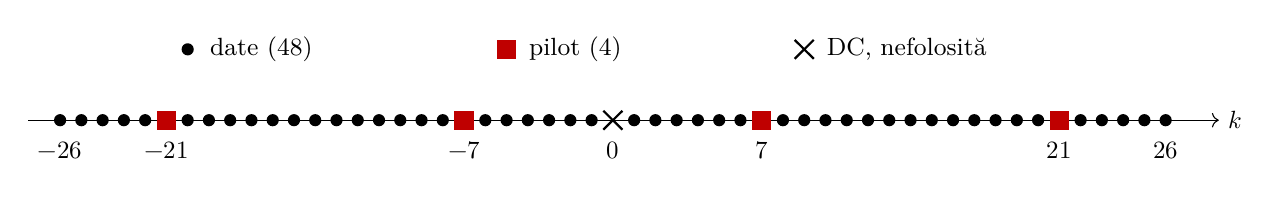
\begin{tikzpicture}[x=0.27cm, y=1cm, font=\small]
		\draw[->] (-27.5,0) -- (28.5,0) node[right] {$k$};
		\foreach \k in {-26,...,-22} \fill (\k,0) circle (2.2pt);
		\foreach \k in {-20,...,-8} \fill (\k,0) circle (2.2pt);
		\foreach \k in {-6,...,-1} \fill (\k,0) circle (2.2pt);
		\foreach \k in {1,...,6} \fill (\k,0) circle (2.2pt);
		\foreach \k in {8,...,20} \fill (\k,0) circle (2.2pt);
		\foreach \k in {22,...,26} \fill (\k,0) circle (2.2pt);
		\foreach \k in {-21,-7,7,21} \fill[red!75!black] (\k-0.45,-0.12) rectangle (\k+0.45,0.12);
		\draw[thick] (-0.45,-0.12) -- (0.45,0.12) (-0.45,0.12) -- (0.45,-0.12);
		\foreach \k in {-26,-21,-7,0,7,21,26} \node[below] at (\k,-0.15) {$\k$};
		\fill (-20,0.9) circle (2.2pt); \node[right] at (-19.4,0.9) {date (48)};
		\fill[red!75!black] (-5.45,0.78) rectangle (-4.55,1.02); \node[right] at (-4.4,0.9) {pilot (4)};
		\draw[thick] (8.55,0.78) -- (9.45,1.02) (8.55,1.02) -- (9.45,0.78); \node[right] at (9.6,0.9) {DC, nefolosită};
	\end{tikzpicture}
	\caption{Așezarea subpurtătoarelor OFDM într-un canal IEEE 802.11a de 20~MHz, după~\cite[Sec.~17.3.2.1]{ieee80211a}. Desen propriu.}
	\label{fig:subpurtatoare}
\end{figure}

În semnalul definit de standard, subpurtătoarea $k$ apare în banda de bază la frecvența $k\Delta_F$~\cite[ec.~(9)]{ieee80211a}.
Prin conversia~\eqref{eq:banda_baza}, ea se află la frecvența radio
\begin{equation}\label{eq:fk}
	f_k = f_c + k\,\Delta_F \qquad \text{(calcul propriu)}.
\end{equation}

Standardul IEEE~802.11a definește aceste valori pentru banda de 5~GHz~\cite{ieee80211a}.
Documentația Espressif pentru ESP32 dă aceeași plajă de subpurtătoare ($-26 \ldots +26$, 52 în total) pentru 802.11a/g.
Pentru 802.11n la 20~MHz, aceeași documentație dă plaja $-28 \ldots +28$, cu 56 de subpurtătoare~\cite{espidf517wifi}.
Halperin et~al. menționează, de asemenea, cele 56 de subpurtătoare ale unui canal 802.11n de 20~MHz~\cite[Sec.~2]{halperin2011}.

%--------------------------------------------------------------------
\section{Estimarea canalului și definiția CSI}\label{sec:estimare}

Ca să demoduleze datele, receptorul trebuie să cunoască $H_n$ din~\eqref{eq:ofdm}.
El îl estimează dintr-o secvență cunoscută, numită secvență pilot sau secvență de antrenare~\cite[Sec.~3.1.2]{tse2005}.
În IEEE~802.11a, această secvență se află în preambulul fiecărui cadru OFDM (figura~\ref{fig:preambul}).

\begin{figure}[ht]
	\centering
	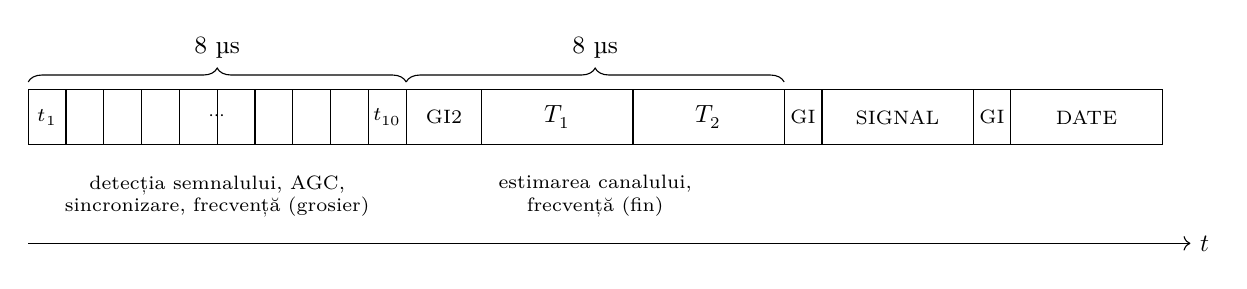
\begin{tikzpicture}[x=0.6cm, y=1cm, font=\small]
		% simbolurile scurte t1..t10, câte 0,8 µs
		\foreach \i in {1,...,10} {
			\draw (\i*0.8-0.8,0) rectangle (\i*0.8,0.7);
		}
		\node at (0.4,0.35) {\scriptsize $t_1$};
		\node at (7.6,0.35) {\scriptsize $t_{10}$};
		\node at (4.0,0.35) {\scriptsize $\cdots$};
		% GI2, T1, T2
		\draw (8,0) rectangle (9.6,0.7); \node at (8.8,0.35) {\scriptsize GI2};
		\draw (9.6,0) rectangle (12.8,0.7); \node at (11.2,0.35) {$T_1$};
		\draw (12.8,0) rectangle (16,0.7); \node at (14.4,0.35) {$T_2$};
		% SIGNAL și DATE
		\draw (16,0) rectangle (16.8,0.7); \node at (16.4,0.35) {\scriptsize GI};
		\draw (16.8,0) rectangle (20,0.7); \node at (18.4,0.35) {\scriptsize SIGNAL};
		\draw (20,0) rectangle (20.8,0.7); \node at (20.4,0.35) {\scriptsize GI};
		\draw (20.8,0) rectangle (24,0.7); \node at (22.4,0.35) {\scriptsize DATE};
		% acolade
		\draw[decorate, decoration={brace, amplitude=5pt}] (0,0.8) -- (8,0.8) node[midway, above=5pt] {8~µs};
		\draw[decorate, decoration={brace, amplitude=5pt}] (8,0.8) -- (16,0.8) node[midway, above=5pt] {8~µs};
		\node[align=center, font=\scriptsize] at (4,-0.65) {detecția semnalului, AGC,\\sincronizare, frecvență (grosier)};
		\node[align=center, font=\scriptsize] at (12,-0.65) {estimarea canalului,\\frecvență (fin)};
		\draw[->] (0,-1.25) -- (24.6,-1.25) node[right] {$t$};
	\end{tikzpicture}
	\caption{Structura preambulului OFDM IEEE 802.11a: zece simboluri scurte ($t_1 \ldots t_{10}$) și două simboluri lungi ($T_1$, $T_2$). Redesenat după~\cite[Fig.~110]{ieee80211a}.}
	\label{fig:preambul}
\end{figure}

Preambulul durează 16~µs și are două părți~\cite[Sec.~17.3.2.1, 17.3.3]{ieee80211a}:
\begin{itemize}
	\item zece simboluri de antrenare scurte, folosite pentru detecția semnalului, convergența controlului automat al amplificării (\emph{Automatic Gain Control}, AGC), selecția diversității, sincronizarea în timp și estimarea grosieră a frecvenței;
	\item două simboluri de antrenare lungi, folosite pentru estimarea canalului și estimarea fină a frecvenței.
\end{itemize}

Simbolul de antrenare lung folosește 53 de subpurtătoare, inclusiv valoarea zero de la frecvența centrală.
Subpurtătoarele sunt modulate cu o secvență cunoscută, $L_k \in \{-1, +1\}$ pentru $k \neq 0$, iar $L_0 = 0$~\cite[ec.~(8)]{ieee80211a}.
Secvența lungă se transmite de două ori, pentru o estimare mai precisă a canalului~\cite[Sec.~17.3.3]{ieee80211a}.

Prin aplicarea relației~\eqref{eq:ofdm} pe subpurtătoarea $k$ a simbolului lung, se obține
\begin{equation}\label{eq:ltf}
	Y_k = H_k L_k + W_k.
\end{equation}
Deoarece $L_k^2 = 1$, o estimare directă a canalului este
\begin{equation}\label{eq:estimare}
	\hat{H}_k = Y_k L_k = H_k + L_k W_k, \qquad k \in \{-26, \ldots, 26\} \setminus \{0\} \qquad \text{(calcul propriu)}.
\end{equation}
Media celor două repetări ale simbolului lung reduce la jumătate varianța zgomotului din estimare, dacă zgomotul celor două repetări este independent (calcul propriu).
Relația~\eqref{eq:estimare} este forma cea mai simplă.
Un receptor real poate folosi și alte metode, care nu sunt descrise în sursele citate.

Halperin et~al. descriu același mecanism la plăcile 802.11n.
Fiecare placă măsoară starea canalului pentru fiecare pachet primit, în timpul preambulului.
Egalizatorul folosește apoi această măsurătoare ca să compenseze efectul canalului înainte de demodulare~\cite[Sec.~2]{halperin2011}.
Estimarea se face pe fiecare subpurtătoare, în domeniul frecvență, din preambulul lung~\cite{chen2016trips}.

\begin{definition}
\emph{Informația despre starea canalului} (CSI) este setul de valori complexe $\hat{H}_k$ care descriu canalul dintre emițător și receptor la nivelul fiecărei subpurtătoare, pentru fiecare pereche de antene de emisie și de recepție~\cite{halperin2011}.
\end{definition}

CSI este deci o versiune eșantionată în frecvență a răspunsului canalului, care leagă semnalul emis și semnalul recepționat prin $Y(f,t) = H(f,t)\, X(f,t)$~\cite[Sec.~3.1]{wang2015carm}.
Pentru o singură pereche de antene și un cadru 802.11a/g, CSI are cel mult 52 de valori complexe, câte una pentru fiecare subpurtătoare folosită (calcul propriu, din tabelul~\ref{tab:ofdm}).

Spre deosebire de CSI, indicatorul puterii semnalului recepționat (\emph{Received Signal Strength Indicator}, RSSI) dă o singură valoare pentru tot pachetul.
Halperin et~al. arată patru legături cu performanțe echivalente, al căror RSSI diferă cu până la 13~dB.
CSI explică diferența: unele subpurtătoare sunt puternic atenuate de fadingul selectiv în frecvență~\cite[Sec.~2]{halperin2011}.

O consecință practică rezultă din mecanismul de mai sus.
Receptorul obține CSI doar din cadrele care conțin preambulul OFDM, câte o măsurătoare pentru fiecare pachet primit~\cite[Sec.~2]{halperin2011}.
Rata măsurătorilor depinde deci de traficul de pe canal (deducție proprie).

Ratele de date ale sistemului OFDM din IEEE~802.11a sunt 6, 9, 12, 18, 24, 36, 48 și 54~Mbit/s~\cite[Sec.~17.1]{ieee80211a}.
Un cadru transmis la altă rată, de exemplu la 1~Mbit/s, nu este un cadru OFDM IEEE~802.11a.
Preambulul din figura~\ref{fig:preambul} aparține cadrelor OFDM, deci un astfel de cadru nu dă CSI din simbolurile lungi (deducție proprie).

%--------------------------------------------------------------------
\section{Efectul unei persoane asupra CSI}\label{sec:persoana}

Activitatea umană modifică canalul.
Ea produce atât atenuarea amplitudinii, cât și deplasări de fază în CSI~\cite[Sec.~3.1]{zhang2015antifall}.
Pentru a descrie acest efect, căile se împart în căi statice și o cale dinamică~\cite[p.~121:7]{zeng2019farsense}.
Componenta statică, $H_s(f)$, cuprinde calea directă și reflexiile pe obiectele fixe.
Componenta dinamică provine din reflexia pe persoana în mișcare.
Pentru o singură cale dinamică~\cite[ec.~(2)]{zeng2019farsense},
\begin{equation}\label{eq:static_dinamic}
	H(f, t) = H_s(f) + A(f, t)\, e^{-j2\pi d(t)/\lambda},
\end{equation}
unde $A(f,t)$ este atenuarea complexă, iar $d(t)$ este lungimea căii dinamice.
Pentru deplasări mici, $A$ se poate considera constantă, deoarece câțiva centimetri schimbă foarte puțin o lungime de ordinul metrilor~\cite[p.~121:7]{zeng2019farsense}.
Când $d(t)$ crește cu o lungime de undă, vectorul $H(f,t)$ face o rotație completă, de $2\pi$, în sensul acelor de ceasornic~\cite[p.~121:7]{zeng2019farsense}.
Figura~\ref{fig:fazori} ilustrează această descompunere în planul complex.

\begin{figure}[ht]
	\centering
	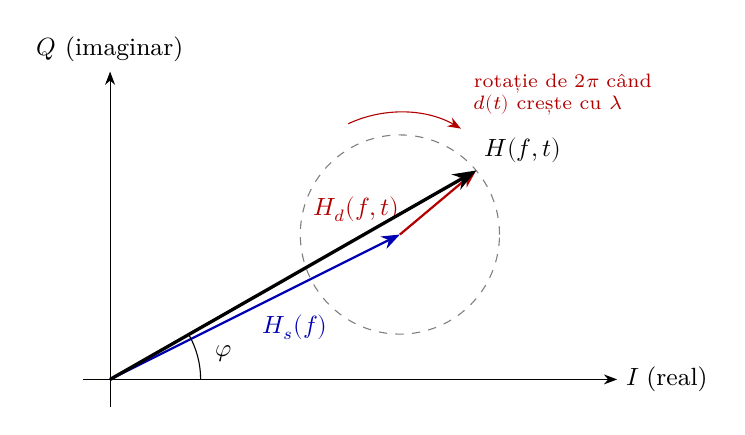
\begin{tikzpicture}[>=Stealth, font=\small, scale=1.15]
		\coordinate (O) at (0,0);
		\coordinate (S) at (3.2,1.6);
		\coordinate (P) at ($(S)+(40:1.1)$);
		% axe
		\draw[->] (-0.3,0) -- (5.6,0) node[right] {$I$ (real)};
		\draw[->] (0,-0.3) -- (0,3.4) node[above] {$Q$ (imaginar)};
		% cercul parcurs de componenta dinamică
		\draw[dashed, gray] (S) circle (1.1);
		% vectori
		\draw[->, thick, blue!70!black] (O) -- (S) node[midway, below right=-1pt] {$H_s(f)$};
		\draw[->, thick, red!70!black] (S) -- (P);
		\node[red!70!black] at ($(S)+(150:0.55)$) {$H_d(f,t)$};
		\draw[->, very thick] (O) -- (P) node[above right=-1pt] {$H(f,t)$};
		% faza vectorului total
		\draw (1.0,0) arc (0:29.7:1.0);
		\node at (1.25,0.28) {$\varphi$};
		% sensul de rotație (în sensul acelor de ceasornic)
		\draw[->, red!70!black] ($(S)+(115:1.35)$) arc (115:60:1.35);
		\node[align=left, font=\scriptsize, red!70!black] at (5.0,3.15) {rotație de $2\pi$ când\\$d(t)$ crește cu $\lambda$};
	\end{tikzpicture}
	\caption{CSI ca sumă dintre o componentă statică și o componentă dinamică, în planul complex. Lungimea vectorului total este amplitudinea $|H|$, iar unghiul $\varphi$ este faza. Desen propriu, după modelul din~\cite{zeng2019farsense,wang2015carm}.}
	\label{fig:fazori}
\end{figure}

Amplitudinea măsurată rezultă din~\eqref{eq:static_dinamic}, cu identitatea $|z_1 + z_2|^2 = |z_1|^2 + |z_2|^2 + 2\,\mathrm{Re}(z_1 z_2^{*})$ (calcul propriu):
\begin{equation}\label{eq:putere}
	|H(f,t)|^2 = |H_s|^2 + |A|^2 + 2\,|H_s|\,|A| \cos\!\left(\frac{2\pi d(t)}{\lambda} + \varphi_0\right), \qquad \varphi_0 = \arg H_s - \arg A.
\end{equation}
Termenul cu cosinus arată că puterea CSI oscilează când persoana se mișcă.
Dacă lungimea căii variază cu viteză constantă, adică $d(t) = d_0 + vt$, oscilația are frecvența $v/\lambda$ (calcul propriu).
De exemplu, la $\lambda \approx 12{,}5$~cm, o cale care se lungește cu 0,5~m/s produce o oscilație de 4~Hz (calcul propriu).
Wang et~al. folosesc aceeași legătură: puterea CFR este o combinație de sinusoide, iar frecvențele acestora, înmulțite cu lungimea de undă, dau vitezele de schimbare ale lungimii căilor~\cite[Sec.~3.4]{wang2015carm}.

În modelul complet al lui Wang et~al., suma căilor este înmulțită cu factorul $e^{-j2\pi\Delta f t}$, produs de diferența $\Delta f$ dintre frecvențele purtătoare ale emițătorului și receptorului~\cite[ec.~(1)]{wang2015carm}.
Acest factor are modulul 1.
El schimbă faza lui $H$, dar nu schimbă amplitudinea $|H|$ (calcul propriu).

%--------------------------------------------------------------------
\section{Limitările măsurării pe echipamente comerciale}\label{sec:limitari}

Faza CSI obținută de la plăcile Wi-Fi comerciale conține mult zgomot.
Cauzele sunt decalajul frecvenței de eșantionare (\emph{Sampling Frequency Offset}, SFO), decalajul frecvenței purtătoare (\emph{Carrier Frequency Offset}, CFO) și întârzierea de detecție a pachetului (\emph{Packet Detection Delay}, PDD).
Din aceste motive, faza brută nu este direct utilizabilă~\cite[p.~121:5]{zeng2019farsense}.
Wang et~al. au măsurat pe plăci comerciale un decalaj de frecvență de aproximativ 80~kHz și erori de fază de până la $0{,}5\pi$.
Aceste erori sunt, în majoritatea cazurilor, mai mari decât schimbările de fază produse de reflexia pe corpul uman~\cite[Sec.~3.3]{wang2015carm}.

Chen et~al. modelează efectele echipamentului astfel~\cite[ec.~(10)]{chen2018trbreath}:
\begin{equation}\label{eq:model_real}
	H_k(t) = \Gamma(t)\,\bigl(S_k(t) + I_k\bigr)\, e^{j(\omega(t) + \kappa(t) k)} + e_k(t).
\end{equation}
Aici $S_k(t)$ este partea utilă a semnalului, produsă de mișcare, iar $I_k$ este partea invariantă în timp, dată de mediul static.
$\Gamma(t)$ este câștigul real al AGC, $\omega(t)$ este distorsiunea inițială de fază, $\kappa(t)$ este distorsiunea liniară de fază, iar $e_k(t)$ este zgomotul termic.
Distorsiunile de fază provin din diferențele dintre oscilatoarele locale ale emițătorului și receptorului.
Variația de amplitudine provine din AGC, care scalează tensiunea de intrare în domeniul dinamic al convertorului analog-numeric~\cite[Sec.~II-C]{chen2018trbreath}.
Simbolurile scurte din preambul servesc chiar la convergența AGC~\cite[Sec.~17.3.2.1]{ieee80211a}, deci câștigul se poate stabili din nou la fiecare cadru (deducție proprie).

Din relația~\eqref{eq:model_real} rezultă trei consecințe (deducție proprie):
\begin{enumerate}
	\item Amplitudinea $|H_k(t)|$ conține factorul $\Gamma(t)$. Valorile absolute ale amplitudinii nu se pot compara direct între momente diferite, dacă AGC și-a schimbat câștigul.
	\item La același moment, raportul amplitudinilor a două subpurtătoare nu depinde de $\Gamma(t)$, dacă zgomotul este mic:
	\begin{equation}\label{eq:raport}
		\frac{|H_{k_1}(t)|}{|H_{k_2}(t)|} \approx \frac{|S_{k_1}(t) + I_{k_1}|}{|S_{k_2}(t) + I_{k_2}|}.
	\end{equation}
	Forma spectrului de amplitudine este deci mai stabilă decât nivelul lui.
	\item Faza conține termenul $\omega(t) + \kappa(t)k$, care variază de la un pachet la altul și crește liniar cu indicele subpurtătoarei. Faza brută trebuie corectată înainte de orice interpretare (secțiunea~\ref{subsec:corectie_faza}).
\end{enumerate}

Eșantionarea în timp are și ea o limitare.
CSI se obține doar când sosește un cadru.
Din cauza traficului Wi-Fi de pe același canal și a pierderii de pachete, momentele de recepție nu sunt echidistante~\cite[Sec.~II-E]{chen2018trbreath}.
O analiză în frecvență a seriei de timp trebuie să țină cont de acest lucru (deducție proprie).

Teorema eșantionării spune că o formă de undă limitată la banda $W/2$ se poate scrie cu eșantioane luate uniform, la intervale de $1/W$~\cite[Sec.~2.2.3]{tse2005}.
Oscilația din~\eqref{eq:putere} are frecvența $v/\lambda$.
Cu o rată de $R$ cadre pe secundă, ea se poate reconstitui doar dacă $v/\lambda \le R/2$, adică $v \le R\lambda/2$ (calcul propriu).
De exemplu, la $\lambda \approx 12{,}5$~cm, rata $R = 100$~cadre/s permite $v \le 6{,}25$~m/s, iar rata $R = 50$~cadre/s permite $v \le 3{,}1$~m/s (calcul propriu).
Relația presupune eșantioane echidistante, deci la eșantionarea neuniformă de mai sus ea este doar orientativă (deducție proprie).

\subsection{Corectarea fazei}\label{subsec:corectie_faza}

Wang, Yang și Mao scriu faza măsurată pe subpurtătoarea $i$ astfel~\cite[ec.~(3)--(4)]{wang2020phasebeat}:
\begin{equation}\label{eq:faza_masurata}
	\widehat{\angle H}_i = \angle H_i + (\epsilon_p + \epsilon_s)\, m_i + \epsilon_c + \beta + Z.
\end{equation}
Aici $\angle H_i$ este faza adevărată, $m_i$ este indicele subpurtătoarei, iar $\epsilon_p$, $\epsilon_s$ și $\epsilon_c$ sunt erorile produse de detecția limitei pachetului, de SFO și de CFO.
$\beta$ este decalajul inițial de fază al buclei cu calare de fază (PLL), iar $Z$ este zgomotul de măsurare.
În sursă, erorile $\epsilon$ sunt notate cu $\lambda$; aici notația este schimbată, ca să nu se confunde cu lungimea de undă.
Valorile acestor erori nu se pot afla și se schimbă de la un pachet la altul.
De aceea, faza adevărată nu se poate obține direct din faza măsurată~\cite[Sec.~2.2]{wang2020phasebeat}.
Relația~\eqref{eq:faza_masurata} are aceeași formă ca termenul $\omega(t) + \kappa(t)k$ din~\eqref{eq:model_real}: o pantă proporțională cu indicele subpurtătoarei și un decalaj comun tuturor subpurtătoarelor (deducție proprie).

Aceeași sursă descrie două metode folosite în literatură pentru a reduce caracterul aleator al fazei~\cite[Sec.~2.2]{wang2020phasebeat}:
\begin{enumerate}
	\item o transformare liniară a fazelor măsurate pe subpurtătoarele unui pachet; scopul ei este eliminarea pantei și a decalajului din~\eqref{eq:faza_masurata} (deducție proprie);
	\item diferența de fază dintre două antene de recepție, din care se scade apoi valoarea medie.
\end{enumerate}
Ambele metode stabilizează faza între pachete consecutive.
Valoarea medie a fazei obținute este însă întotdeauna aproape de zero, deci diferită de faza reală a semnalului~\cite[Sec.~2.2]{wang2020phasebeat}.
În plus, corectarea fazei poate elimina și deplasările de fază produse de mișcarea corpului~\cite[Sec.~3.3]{wang2015carm}.
A doua metodă cere CSI măsurat în același timp pe două antene de recepție (deducție proprie).

%--------------------------------------------------------------------
\section{Obținerea CSI pe ESP32}\label{sec:esp32}

Pe ESP32, CSI este format din răspunsurile în frecvență ale subpurtătoarelor și este estimat când se primesc pachete de la emițător~\cite{espidf517wifi}.
Fiecare valoare complexă ocupă doi octeți cu semn: primul este partea imaginară, al doilea este partea reală~\cite{espidf517wifi}.
Un cadru poate avea până la trei câmpuri din care se obține CSI: câmpul de antrenare lung clasic (\emph{legacy long training field}, LLTF), câmpul de antrenare lung HT (HT-LTF) și câmpul HT-LTF pentru codarea spațiu-timp (STBC-HT-LTF)~\cite{espidf517wifi}.
Câmpurile HT-LTF și STBC-HT-LTF apar doar la cadrele HT, adică 802.11n~\cite{espidf517wifi}.
LLTF corespunde simbolurilor lungi $T_1$ și $T_2$ din figura~\ref{fig:preambul} (deducție proprie).

Pentru LLTF, valorile sunt așezate în ordinea subpurtătoarelor $0 \ldots 31$, apoi $-32 \ldots -1$~\cite{espidf517wifi}.
Aceasta este ordinea intrărilor IFFT din secțiunea~\ref{sec:ofdm}.
Deci pozițiile $0$ și $27 \ldots 37$ din șirul CSI corespund subpurtătoarelor fără semnal (calcul propriu).
Dacă indicatorul \texttt{first\_\allowbreak{}word\_\allowbreak{}invalid} este adevărat, primii patru octeți din CSI sunt invalizi, din cauza unei limitări hardware a ESP32~\cite{espidf517wifi}.
Pentru LLTF, acești patru octeți corespund subpurtătoarelor $0$ și $1$ (calcul propriu).

Documentația cere patru pași: activarea CSI în configurația proiectului, înregistrarea unei funcții de recepție, configurarea CSI și pornirea CSI~\cite{espidf517wifi}.
Configurarea alege câmpurile LLTF, HT-LTF și STBC-HT-LTF.
Dacă un câmp nu este activat, numărul total de octeți CSI scade~\cite{espidf517wifi}.
Funcția de recepție rulează în task-ul Wi-Fi, deci nu trebuie să facă operații lungi.
Datele se pun într-o coadă și se prelucrează într-un task cu prioritate mai mică~\cite{espidf517wifi}.
O stație conectată primește doar pachetele de la AP, deci documentația recomandă modul \emph{sniffer} (promiscuu), pentru mai multe măsurători CSI~\cite{espidf517wifi}.

Bibliotecile Wi-Fi ale ESP-IDF sunt livrate fără cod sursă.
Dezasamblarea lor arată următorul lanț (analiză proprie):
\begin{enumerate}
	\item funcțiile de configurare nu scriu direct în regiștri; ele trimit un mesaj task-ului Wi-Fi, care face modificarea;
	\item funcția \texttt{hal\_\allowbreak{}mac\_\allowbreak{}set\_\allowbreak{}csi} pornește CSI: ea pune pe 1 bitul 23 din registrul \texttt{0x3FF7309C};
	\item funcția \texttt{phy\_\allowbreak{}chan\_\allowbreak{}dump\_\allowbreak{}cfg} configurează CSI: ea scrie alegerea câmpurilor LTF și scalarea valorilor în registrul \texttt{0x3FF5CD0C};
	\item funcția \texttt{wdev\_\allowbreak{}csi\_\allowbreak{}rx\_\allowbreak{}process} rulează la fiecare cadru: ea completează structura \texttt{wifi\_\allowbreak{}csi\_\allowbreak{}info\_\allowbreak{}t} și apelează funcția de recepție a aplicației.
\end{enumerate}
Biblioteca nu calculează estimarea; ea predă aplicației un rezultat gata calculat (analiză proprie).
Deci estimarea canalului din secțiunea~\ref{sec:estimare} se face în hardware (deducție proprie).
Algoritmul exact al estimării nu este public.

%--------------------------------------------------------------------
\section{Sinteză}\label{sec:sinteza}

Tabelul~\ref{tab:sinteza} rezumă mărimile care se pot obține din CSI, ce descriu ele și limitarea principală a fiecăreia, conform secțiunilor anterioare.

\begin{table}[ht]
	\caption{Mărimi obținute din CSI și limitările lor}
	\centering
	\begin{tabular}{|p{3.4cm}|p{5.6cm}|p{5.2cm}|}
		\hline
		Mărime & Ce descrie & Limitare principală \\
		\hline
		Amplitudinea $|H_k|$ & suma căilor pe subpurtătoarea $k$, ec.~\eqref{eq:cfr} & scalată de AGC, ec.~\eqref{eq:model_real} \\
		\hline
		Raportul $|H_{k_1}|/|H_{k_2}|$ & forma spectrului de amplitudine & nu dă nivelul absolut, ec.~\eqref{eq:raport} \\
		\hline
		Faza $\varphi_k$ & lungimea căilor ($2\pi$ la fiecare $\lambda$) & CFO, SFO, PDD; trebuie corectată, ec.~\eqref{eq:faza_masurata} \\
		\hline
		Variația în timp a lui $|H|^2$ & viteza de schimbare a lungimii căii dinamice ($v/\lambda$), ec.~\eqref{eq:putere} & eșantionare neuniformă în timp \\
		\hline
		RSSI & puterea întregului cadru & o singură valoare, fără detaliu pe frecvență \\
		\hline
	\end{tabular}
	\label{tab:sinteza}
\end{table}
 % \chapter{Analiză și Fundamentare Teoretică}

\chapter{Proiectare de detaliu și implementare}\label{ch:proiectare}
\pagestyle{fancy}

\notalucru{De scris: schema generală a aplicației și descrierea fiecărei componente (firmware ESP32, interfața pe PC).}
 % \chapter{Proiectare de Detaliu și Implementare}

\chapter{Testare și validare}\label{ch:testare}
\pagestyle{fancy}

\notalucru{De scris: descrierea datelor măsurate și a testelor, fără o ipoteză de dovedit.}
 % \chapter{Testare și Validare}

\chapter{Manual de instalare și utilizare}\label{ch:instalare}
\pagestyle{fancy}

\notalucru{De scris (1--5 pagini): resursele hardware și software, instalarea pas cu pas și utilizarea.}
 % \chapter{Manual de Instalare și Utilizare}

\chapter{Concluzii}\label{ch:concluzii}
\pagestyle{fancy}

\notalucru{De scris (1--2 pagini): rezumatul contribuțiilor, analiza critică a rezultatelor, dezvoltări ulterioare.}
 % \chapter{Concluzii}

\bibliographystyle{IEEEtran}
\bibliography{licenta}%same file name as for .bib

\appendix
\chapter{Secțiuni relevante din cod}
\pagestyle{fancy}

\notalucru{De completat la final.}


\end{document}
